%!TEX spellcheck=ro_RO
%!TEX root = ./main.tex
\chapter{Prezentarea aplicației}\label{ch:3implementare}

\textbf{Note implementare:}
\begin{enumerate}
\item Diferite incercari de a extrage feateruri
\item Probleme intampinate in asemanarea datelor NEUTRAL si RELAXED
\item Uita-te pe notebooku Licenta\_CNN
\end{enumerate}

Scopul lucrării îl constituie folosirea paradigmei învățării automate supervizate, mai precis, utilizarea rețelelor neuronale convoluționale pentru clasificarea a trei stări mentale diferite, și anume: \textit{neutru, relaxat} și \textit{concentrat}. 

Datele aferente fiecărei stări provin de la un dispozitiv comercial, \textit{Muse 2016}, capabil de a înregistra activitatea cerebrală folosind tehnica de imagistică \textbf{EEG} \textit{(Electroencefalografia)}, neinvazivă. Aceste înregistrări reprezintă activitatea creierului din jurul electrozilor dispusă în timp. Deoarece dispozitivul folosit folosește o tehnică neinvazivă cu electrozi uscați datele finale ale înregistrării conțin zgomot produs de mișcările persoanei, de contracțiile mușchilor sau chiar de clipit. Din aceste motive datele trebuie prelucrate. Este de menționat faptul că nu există o anumită formulă de prelucrare pentru ca datele sa fie perfecte pentru etapa de clasificare, metodele folosite în această etapă fiind stabilite adesea empiric. După prelucrarea datelor, urmează un pas de extragere a anumitor atribute/caracteristici statistice și spectrale pe baza cărora vor fi construite imaginile alb-negru. Fiecare imagine va avea o etichetă aferentă clasei din care face parte, neutru, relaxat sau concentrat.

După etapa de prelucrare și etichetare a datelor, urmează pregătirea datelor pentru transformarea acestora sub forma unor imagini alb-negru. Această etapă include selectarea celor mai relevante 400 de atribute, dintr-un total de 414. Pentru a putea fi folosite ca și componente ale unei imagini alb-negru, este necesară normalizarea datelor în intervalul $[0,1]$, 0 reprezentând negru, 1 reprezentând alb, orice altă valoare aparținând intervalului reprezentând o nuanță de gri. Imaginile sunt împărțite apoi în diferite seturi, fiecare cu scopul său specific; setul de antrenare, setul de validare și setul de testare. Antrenarea rețelei convoluționale se realizează folosind setul de antrenare și setul de validare pentru evaluarea performanțelor pe parcursul antrenării. În final, setul de testare este folosit pentru a determina performanța rețelei pe date complet noi, rezultând metricile finale, precum acuratețea sau valoarea funcției de cost \textit{(loss)}. În cazul rețelei dezvoltate în această lucrare a fost atinsă o acuratețe de $\approx91.83\%$ cu valoarea funcției de loss de $\approx0.2511$

În continuarea capitolului, etapele prezentate sumar anterior vor fi detaliate și explicate, iar la finalul capitolului vor fi prezentate rezultatele diferitor implementări și menționate problemele apărute pe parcursul implementării.

\section{Etape implementare}

\subsection{Achiziție date}

\textbf{Note implementare:}
\begin{enumerate}
\item Cu ce device am achizitionat datele, detalii despre el, plasarea senzorilor (standardul + poza standard)
\item Eventual detalii despre BLE
\item Cum am achizitionat datele, numar persoane + detalii despre stari, durata inregistrarilor, 2x inregistrari/persoana, poza muselsl date initiale
\item  Detalii despre datele culese
\end{enumerate}

Pentru achiziția datelor a fost folosită casca comercial valabilă Muse 2016. Aceasta conține cinci electrozi uscați, unul fiind folosit ca punct de referință, iar ceilalți patru pentru a înregistra semnalele EEG. Electrozii sunt poziționați în locațiile \textit{TP9, AF7, Fpz, AF8, TP10}, conform unei versiuni modificate a sistemului internațional 10-20 de poziționare al electrozilor EEG. Electrodul Fpz este folosit ca electrod de referință. În \autoref{fig:eegstandard} este prezentat aranjamentul electrozilor.

\begin{figure}[ht]
\centering
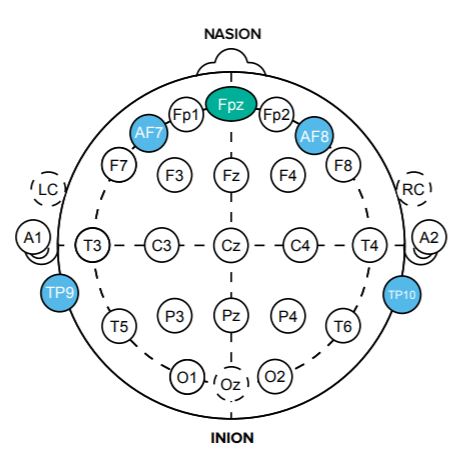
\includegraphics[width=10cm, keepaspectratio]{fig/cap3/EEGstandard.png}
\caption{Versiunea modificată a sistemului internațional 10-20 împreună cu marcajul poziției electrozilor căștii Muse \cite{online:muse-eeg}.}
\label{fig:eegstandard}
\end{figure}

Datele EEG au fost colectate de la 12 persoane. \textbf{TODO CONTINUARE}

Pentru a diminua zgomotul înregistrat de senzori, pentru fiecare stare au fost alese activități care necesitau o mișcare minimă a persoanei examinate. Citirile datelor de la electrozii AF7 și AF8, fiind situați pe frunte, sunt distorsionate de mișcările generate de clipit. Astfel, pentru a păstra o uniformitate asupra celor trei stări, clipitul nu a fost nici încurajat nici descurajat. Chiar dacă acesta este considerat zgomot, rata de clipire este influențată de starea de concentrare a persoanei, acest lucru fiind util în final pentru algoritmul de clasificare. Totuși, persoanelor examinate le-a fost specificat să nu inchidă ochii pe durata unui test.

Pentru determinarea celor trei stări mentale, au fost stabilite trei activități, conform \cite{eeg:2018}. Pentru înregistrarea stării neutre, participanții au fost îndrumați să păstreze o poziție confortabilă a corpului și o stare mentală echilibrată, nici prea relaxată dar nici prea activă. Înregistrarea stării mentale de relaxare a presupus ca subiecții să asculte o piesă muzicală cu o tonalitate și un tempo scăzut. Acestora le-a fost indicat faptul de a se relaxa complet, atât fizic cât și psihic. Pentru determinarea unei stări mentale active și concentrate participanții au fost instruiți să joace jocul „alba-neagra”, în care un obiect este ascuns sub unul din mai multe pahare care mai apoi sunt amestecate între ele. Scopul fiind de a identifica paharul care conține obiectul. Pe parcursul jocului, numărul paharelor și viteza cu care acestea se mișcă va crește.

\subsection{Preprocesare date}

\subsection{Arhitectura rețelei}

\subsection{Antrenarea rețelei}

\subsection{Evaluarea și ajustarea parametrilor}

\section{Rezultate}
